\subsection{Command}
Viene utilizzato per incapsulare delle richieste all'interno di un oggetto, in modo che il client siano indipendenti dal tipo di richiesta.

\begin{figure}[ht]
    \centering
    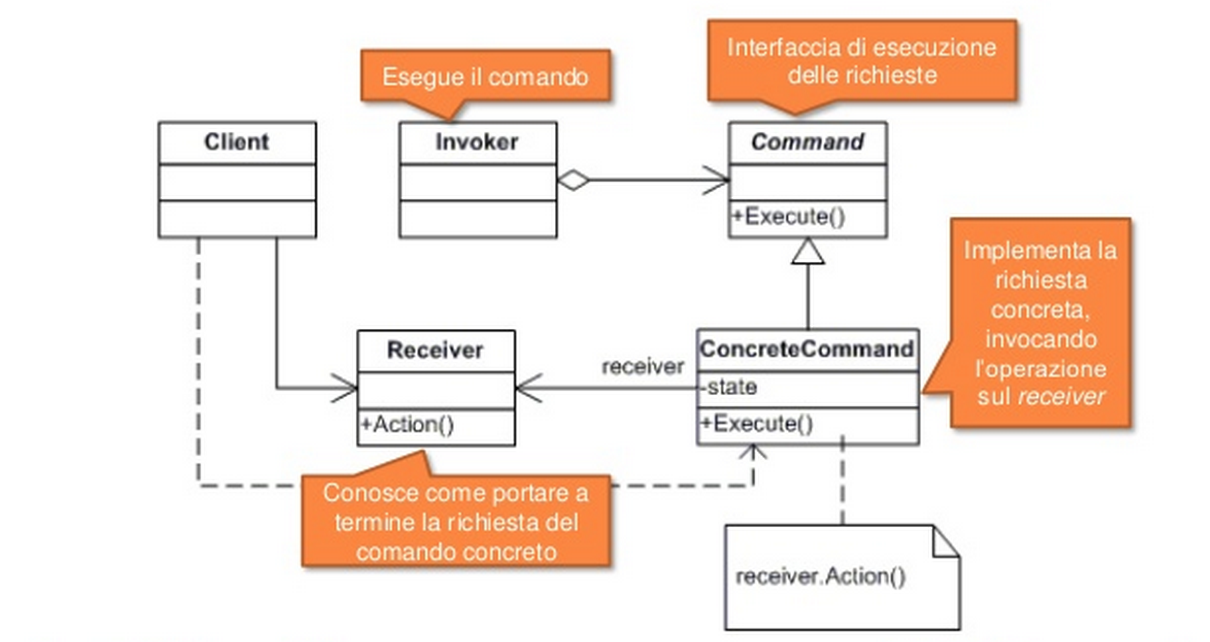
\includegraphics[width=0.8\textwidth]{immagini/command.png}
    \caption{Command}
\end{figure}
\FloatBarrier

\subsubsection{Utilizzo}
\begin{enumerate}
\item Il client crea il comando da eseguire;
\item Il client passa il comando da eseguire all'invoker (oggetto che si occupa di gestire i comandi);
\item L'invoker eseguire il comando, producendo degli effetti sul reciver.
\end{enumerate}
\begin{figure}[ht]
    \centering
    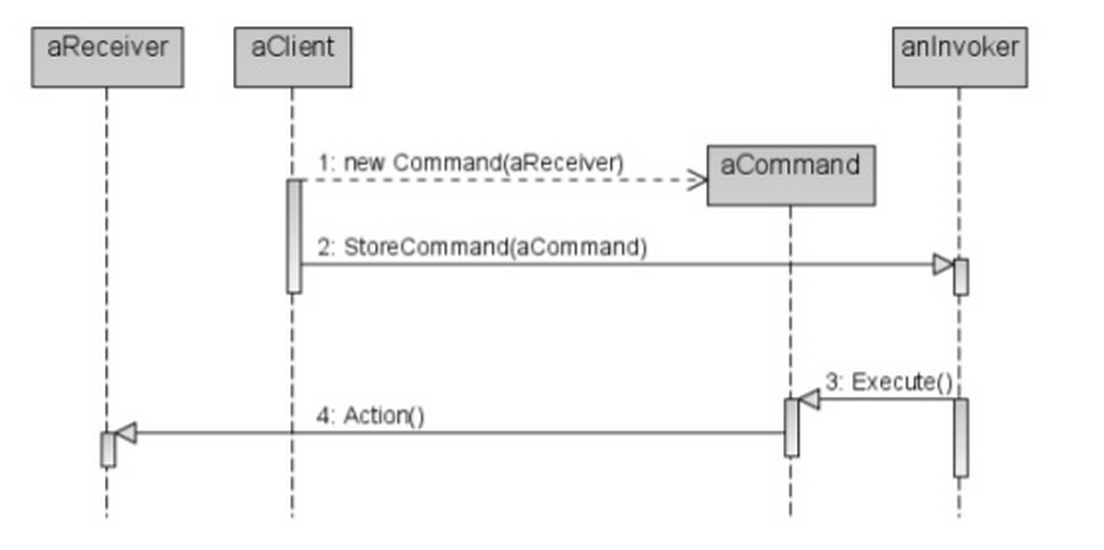
\includegraphics[width=0.8\textwidth]{immagini/commandSequence.png}
    \caption{Diagramma di sequenza - Command pattern}
\end{figure}
\FloatBarrier


\subsubsection{Casi tipici}
\begin{itemize}
\item Sono necessarie delle funzionalità di callback;
\item Le richieste devono essere gestite in momenti differenti o in ordine diverso;
\item \`{E} necessario tenere uno storico delle richieste effettuate;
\item Tra il chiamante e il ricevente deve esserci un accoppiamento lasco.
\end{itemize}